\documentclass[12pt,a4paper,pagesize=pdftex]{scrartcl}
\usepackage[latin1]{inputenc}
\usepackage[english]{babel}
\usepackage{amsmath}
\usepackage{amsthm}
\usepackage{amssymb}
\usepackage{lmodern}
\usepackage{color}
\usepackage{graphicx}
\usepackage{caption}
\usepackage{textcomp}
\usepackage{gensymb}
\usepackage{listings}
\usepackage{units}
\usepackage{hyperref}
\usepackage{float}
\lstset{frame = single, breaklines=true, postbreak=\raisebox{0ex}[0ex][0ex]
{\ensuremath{\color{red}\hookrightarrow\space}}}
\usepackage[pass,letterpaper]{geometry}
\usepackage[section]{placeins}
\graphicspath{ {.} }
\renewcommand{\thesubsection}{\thesection\alph{subsection}}
\title{Numerical Solution and Implementation of the Jointly Markovian Probability Master Equations}
\subtitle{}
\author{}
\date{}
\linespread{1.25}

\begin{document}

\pdfpageheight 11in
\pdfpagewidth 8.5in

\maketitle

% BEGIN DOCUMENT
\section*{Probability Master Equations}
The probability master equations start as a coupled system of two equations with non-constant coefficients dependent on the \(\phi\) and \(\theta\) domains:

\begin{multline*}
    \frac{\partial}{\partial t} \left(p_1 P_1 \left(\phi, \theta, t\right)\right) + \frac{\partial}{\partial \phi} \left(f_1\left(\phi, \theta\right) p_1 P_1 \left(\phi, \theta, t\right)\right) + \frac{\partial}{\partial \theta} \left(g_1 \left(\phi, \theta\right) p_1 P_1\left(\phi, \theta, t\right)\right) \\= \frac{p_2}{\tau_2} P_2 \left(\phi, \theta, t\right) - \frac{p_1}{\tau_1} P_1\left(\phi, \theta, t\right)
\end{multline*}

\begin{multline*}
    \frac{\partial}{\partial t} \left(p_2 P_2 \left(\phi, \theta, t\right) \right) + \frac{\partial}{\partial \phi} \left(f_2 \left(\phi, \theta\right) p_2 P_2 \left(\phi, \theta, t\right)\right) + \frac{\partial}{\partial \theta} \left(g_2 \left(\phi, \theta\right) p_2 P_2\left(\phi, \theta, t\right)\right) \\= \frac{p_1}{\tau_1} P_1\left(\phi, \theta, t\right) - \frac{p_2}{\tau_2} P_2\left(\phi, \theta, t\right)
\end{multline*}

Initial conditions are defined in terms of radiation intensity and material temperature through the use of the Dirac delta function as:

\begin{equation*}
    P_i\left(\phi, \theta, 0\right) = \delta\left(\phi - I_0\right) \delta\left(\theta - T_0\right), \quad i = 1, 2
\end{equation*}

In these equations, \(f\) and \(g\) represent non-constant coefficients from material energy balance constraints, and are defined as follows:

\begin{equation*}
    f_i\left(\phi, \theta\right) = c \sigma_{a,i}\left(\theta\right) \left(c a \theta^4 - \phi\right), \quad i = 1, 2
\end{equation*}

\begin{equation*}
    g_i\left(\phi, \theta\right) = \frac{\sigma_{a,i}\left(\theta\right)}{\rho_i\left(\theta\right)c_{v,i}\left(\theta\right)}\left(\phi - c a \theta^4\right), \quad i = 1, 2
\end{equation*}

We can start the derivation of numerical methods by folding the volume fraction term into the appropriate term for the conditional probability density. Thus, moving forward, the notation of \(P_1\) and \(P_2\) will refer to the products \(p_1 P_1\) and \(p_2 P_2\), respectively. For the purposes of this analysis, the initial volume fractions are constants and may be safely accounted for at the conclusion of numerical calculation to obtain the correct conditional probability density.

The first approach is to apply a simple Backwards-Euler linearization approximation to the time derivative in these equations, allowing for an implicit system to be computed at each discrete time-step. This is relevant for all means of numerical analysis approached herein. The time-step notation will be represented by the index \(n\) in the form of a superscript.

\begin{multline*}
    \frac{1}{\Delta t} \left(P^{n+1}_1\left(\phi, \theta, t\right) - P^n_1\left(\phi, \theta, t\right)\right) + \frac{\partial}{\partial \phi} \left(f_1\left(\phi, \theta, t\right) P_1^{n+1} \left(\phi, \theta, t\right) \right) \\+ \frac{\partial}{\partial \theta} \left(g_1 \left(\phi, \theta, t\right) P_1^{n+1} \left(\phi, \theta, t\right)\right) = \frac{1}{\tau_2} P_2^{n+1}\left(\phi, \theta, t\right) - \frac{1}{\tau_1}P_1^{n+1}\left(\phi, \theta, t\right)
\end{multline*}

\begin{multline*}
    \frac{1}{\Delta t} \left(P^{n+1}_2\left(\phi, \theta, t\right) - P^n_2\left(\phi, \theta, t\right)\right) + \frac{\partial}{\partial \phi} \left(f_2\left(\phi, \theta, t\right) P_2^{n+1} \left(\phi, \theta, t\right) \right) \\+ \frac{\partial}{\partial \theta} \left(g_2 \left(\phi, \theta, t\right) P_2^{n+1} \left(\phi, \theta, t\right)\right) = \frac{1}{\tau_1} P_1^{n+1}\left(\phi, \theta, t\right) - \frac{1}{\tau_2}P_2^{n+1}\left(\phi, \theta, t\right)
\end{multline*}

We can factor the \(\Delta t\) term across the equation to allow for isolation of the previous time-step value.

\begin{multline*}
    P_1^{n+1}\left(\phi, \theta, t\right) - P_1^n\left(\phi, \theta, t\right) + \Delta t \frac{\partial}{\partial \phi} \left(f_1 \left(\phi, \theta, t\right) P_1^{n+1} \left(\phi, \theta, t\right)\right) \\+ \Delta t\frac{\partial}{\partial \theta} \left(g_1 \left(\phi, \theta, t\right) P_1^{n+1} \left(\phi, \theta, t\right)\right) = \frac{\Delta t}{\tau_2} P_2^{n+1}\left(\phi, \theta, t\right) - \frac{\Delta t}{\tau_1} P_1^{n+1} \left(\phi, \theta, t\right)
\end{multline*}

\begin{multline*}
    P_2^{n+1}\left(\phi, \theta, t\right) - P_2^n\left(\phi, \theta, t\right) + \Delta t \frac{\partial}{\partial \phi} \left(f_2 \left(\phi, \theta, t\right) P_2^{n+1} \left(\phi, \theta, t\right)\right) \\+ \Delta t\frac{\partial}{\partial \theta} \left(g_2 \left(\phi, \theta, t\right) P_2^{n+1} \left(\phi, \theta, t\right)\right) = \frac{\Delta t}{\tau_1} P_1^{n+1}\left(\phi, \theta, t\right) - \frac{\Delta t}{\tau_2} P_2^{n+1} \left(\phi, \theta, t\right)
\end{multline*}

\newpage
\section*{Finite Difference}

Generic central-difference formula:

\begin{equation*}
    f^\prime \left(x_i\right) \approx \frac{f\left(x_{i+1}\right) - f\left(x_{i-1}\right)}{2 \Delta x}
\end{equation*}

The most straightforward numerical method to implement is the finite central-difference model, which involves linearizing and discretizing in both the \(\phi\) and \(\theta\) dimensions, represented by subscript \(i\) and \(j\) for cellular indices, respectively. For brevity in this notation, the \(\phi\), \(\theta\), and \(t\) dependence in these equations is omitted.

\begin{multline*}
    P_{1,i,j}^{n+1} - P_{1,i,j}^n + \frac{\Delta t}{2 \Delta \phi} \left(f_{1,i+1,j}P^{n+1}_{1,i+1,j} - f_{1,i-1,j}P^{n+1}_{1,i-1,j}\right) \\+ \frac{\Delta t}{2 \Delta \theta} \left(g_{1,i,j+1} P^{n+1}_{1,i,j+1} - g_{1,i,j-1} P^{n+1}_{1,i,j-1}\right) = \frac{\Delta t}{\tau_2} P^{n+1}_{2,i,j} - \frac{\Delta t}{\tau_1}P^{n+1}_{1,i,j}
\end{multline*}

\begin{multline*}
    P_{2,i,j}^{n+1} - P_{2,i,j}^n + \frac{\Delta t}{2 \Delta \phi} \left(f_{2,i+1,j}P^{n+1}_{2,i+1,j} - f_{2,i-1,j}P^{n+1}_{2,i-1,j}\right) \\+ \frac{\Delta t}{2 \Delta \theta} \left(g_{2,i,j+1} P^{n+1}_{2,i,j+1} - g_{2,i,j-1} P^{n+1}_{2,i,j-1}\right) = \frac{\Delta t}{\tau_1} P^{n+1}_{1,i,j} - \frac{\Delta t}{\tau_2}P^{n+1}_{2,i,j}
\end{multline*}

This can be expanded into each term and algebraically rewritten with the goal of isolating the \(n\)-th step cell-centered probability density:

\begin{multline*}
    \left(1 + \frac{\Delta t}{\tau_1}\right) P^{n+1}_{1,i,j} - \frac{\Delta t}{\tau_2} P^{n+1}_{2,i,j} + \frac{\Delta t}{2 \Delta \phi} f_{1,i+1,j}P^{n+1}_{1,i+1,j} - \frac{\Delta t}{2 \Delta \phi} f_{1,i-1,j}P^{n+1}_{1,i-1,j} \\+ \frac{\Delta t}{2 \Delta \theta} g_{1,i,j+1} P^{n+1}_{1,i,j+1} - \frac{\Delta t}{2\Delta \theta} g_{1,i,j-1} P^{n+1}_{1,i,j-1} = P^n_{1,i,j}
\end{multline*}

\begin{multline*}
    \left(1 + \frac{\Delta t}{\tau_2}\right) P^{n+1}_{2,i,j} - \frac{\Delta t}{\tau_1} P^{n+1}_{1,i,j} + \frac{\Delta t}{2 \Delta \phi} f_{2,i+1,j}P^{n+1}_{2,i+1,j} - \frac{\Delta t}{2 \Delta \phi} f_{2,i-1,j}P^{n+1}_{2,i-1,j} \\+ \frac{\Delta t}{2 \Delta \theta} g_{2,i,j+1} P^{n+1}_{2,i,j+1} - \frac{\Delta t}{2\Delta \theta} g_{2,i,j-1} P^{n+1}_{2,i,j-1} = P^n_{2,i,j}
\end{multline*}

\subsection*{Boundaries}
At the boundaries, the forward-difference and backward-difference equations are applied, so as to appropriately account for boundary conditions.

\subsubsection*{Forward-Difference}
Generic forward-difference formula:

\begin{equation*}
    f^\prime\left(x\right) \approx \frac{f\left(x_{i+1}\right) - f\left(x_i\right)}{\Delta x}
\end{equation*}

This approximation results in the "bottom-left" corner-case \(\left(0,0\right)\) boundary-value equations:

\begin{multline*}
    \left(1 + \frac{\Delta t}{\tau_1} - \frac{\Delta t}{\Delta \phi} f_{1,0,0} - \frac{\Delta t}{\Delta \theta}g_{1,0,0}\right) P^{n+1}_{1,0,0} - \frac{\Delta t}{\tau_2} P^{n+1}_{2,0,0} \\+ \frac{\Delta t}{\Delta \phi} f_{1,1,0} P^{n+1}_{1,1,0} + \frac{\Delta t}{\Delta \theta} g_{1,0,1} P^{n+1}_{1,0,1} = P^n_{1,0,0}
\end{multline*}

\begin{multline*}
    \left(1 + \frac{\Delta t}{\tau_2} - \frac{\Delta t}{\Delta \phi} f_{2,0,0} - \frac{\Delta t}{\Delta \theta}g_{2,0,0}\right) P^{n+1}_{2,0,0} - \frac{\Delta t}{\tau_1} P^{n+1}_{1,0,0} \\+ \frac{\Delta t}{\Delta \phi} f_{2,1,0} P^{n+1}_{2,1,0} + \frac{\Delta t}{\Delta \theta} g_{2,0,1} P^{n+1}_{2,0,1} = P^n_{2,0,0}
\end{multline*}

The "left" \(\phi\)-edge-case \(\left(0,j\right)\) boundary-value equations:

\begin{multline*}
    \left(1 + \frac{\Delta t}{\tau_1} - \frac{\Delta t}{\Delta \phi} f_{1,0,j}\right) P^{n+1}_{1,0,j} - \frac{\Delta t}{\tau_2} P^{n+1}_{2,0,j} \\+ \frac{\Delta t}{\Delta \phi} f_{1,1,j} P^{n+1}_{1,1,j} + \frac{\Delta t}{2 \Delta \theta} g_{1,0,j+1} P^{n+1}_{1,0,j+1} - \frac{\Delta t}{2 \Delta \theta}g_{1,0,j-1} P^{n+1}_{1,0,j-1} = P^n_{1,0,j}
\end{multline*}

\begin{multline*}
    \left(1 + \frac{\Delta t}{\tau_2} - \frac{\Delta t}{\Delta \phi} f_{2,0,j}\right) P^{n+1}_{2,0,j} - \frac{\Delta t}{\tau_1} P^{n+1}_{1,0,j} \\+ \frac{\Delta t}{\Delta \phi} f_{2,1,j} P^{n+1}_{2,1,j} + \frac{\Delta t}{2 \Delta \theta} g_{2,0,j+1} P^{n+1}_{2,0,j+1} - \frac{\Delta t}{2 \Delta \theta}g_{2,0,j-1} P^{n+1}_{2,0,j-1} = P^n_{2,0,j}
\end{multline*}

And the "bottom" \(\theta\)-edge-case \(\left(i,0\right)\) boundary-value equations:

\begin{multline*}
    \left(1 + \frac{\Delta t}{\tau_1} - \frac{\Delta t}{\Delta \theta}g_{1,i,0}\right)P^{n+1}_{1,i,0} - \frac{\Delta t}{\tau_2}P^{n+1}_{2,i,0} \\+ \frac{\Delta t}{2 \Delta \phi} f_{1,i+1,0} P^{n+1}_{1,i+1,0} - \frac{\Delta t}{2 \Delta \phi} f_{1,i-1,0} P^{n+1}_{1,i-1,0} + \frac{\Delta t}{\Delta \theta} g_{1,i,1} P^{n+1}_{1,i,1} = P^n_{1,i,0}
\end{multline*}

\begin{multline*}
    \left(1 + \frac{\Delta t}{\tau_2} - \frac{\Delta t}{\Delta \theta}g_{2,i,0}\right)P^{n+1}_{2,i,0} - \frac{\Delta t}{\tau_1}P^{n+1}_{1,i,0} \\+ \frac{\Delta t}{2 \Delta \phi} f_{2,i+1,0} P^{n+1}_{2,i+1,0} - \frac{\Delta t}{2 \Delta \phi} f_{2,i-1,0} P^{n+1}_{2,i-1,0} + \frac{\Delta t}{\Delta \theta} g_{2,i,1} P^{n+1}_{2,i,1} = P^n_{2,i,0}
\end{multline*}

\subsubsection*{Backward-Difference}
Generic backward-difference formula:

\begin{equation*}
    f^\prime\left(x\right) \approx \frac{f\left(x_i\right) - f\left(x_{i-1}\right)}{\Delta x}
\end{equation*}

This approximation results in the "top-right" corner-case \(\left(\Phi,\Theta\right)\) boundary-value equations:

\begin{multline*}
    \left(1 + \frac{\Delta t}{\tau_1} + \frac{\Delta t}{\Delta \phi} f_{1,\Phi,\Theta} + \frac{\Delta t}{\Delta \theta} g_{1,\Phi,\Theta}\right) P^{n+1}_{1,\Phi,\Theta} - \frac{\Delta t}{\tau_2} P^{n+1}_{2,\Phi,\Theta} \\- \frac{\Delta t}{\Delta \phi} f_{1,\Phi-1,\Theta} P^{n+1}_{1,\Phi-1,\Theta} - \frac{\Delta t}{\Delta \theta} g_{1,\Phi,\Theta-1} P^{n+1}_{1,\Phi,\Theta-1} = P^n_{1,\Phi,\Theta}
\end{multline*}

\begin{multline*}
    \left(1 + \frac{\Delta t}{\tau_2} + \frac{\Delta t}{\Delta \phi} f_{2,\Phi,\Theta} + \frac{\Delta t}{\Delta \theta} g_{2,\Phi,\Theta}\right) P^{n+1}_{2,\Phi,\Theta} - \frac{\Delta t}{\tau_1} P^{n+1}_{1,\Phi,\Theta} \\- \frac{\Delta t}{\Delta \phi} f_{2,\Phi-1,\Theta} P^{n+1}_{2,\Phi-1,\Theta} - \frac{\Delta t}{\Delta \theta} g_{2,\Phi,\Theta-1} P^{n+1}_{2,\Phi,\Theta-1} = P^n_{2,\Phi,\Theta}
\end{multline*}

The "right" \(\phi\)-edge-case \(\left(\Phi,j\right)\) boundary-value equations:

\begin{multline*}
    \left(1 + \frac{\Delta t}{\tau_1} + \frac{\Delta t}{\Delta \phi}f_{1,\Phi,j}\right) P^{n+1}_{1,\Phi,j} - \frac{\Delta t}{\tau_2} P^{n+1}_{2,\Phi,j} \\- \frac{\Delta t}{\Delta \phi} f_{1,\Phi-1,j} P^{n+1}_{1,\Phi-1,j} + \frac{\Delta t}{2 \Delta \theta} g_{1,\Phi,j+1} P^{n+1}_{1,\Phi,j+1} - \frac{\Delta t}{2 \Delta \theta} g_{1,\Phi,j-1} P^{n+1}_{1,\Phi,j-1} = P^n_{1,\Phi,j}
\end{multline*}

\begin{multline*}
    \left(1 + \frac{\Delta t}{\tau_2} + \frac{\Delta t}{\Delta \phi}f_{2,\Phi,j}\right) P^{n+1}_{2,\Phi,j} - \frac{\Delta t}{\tau_1} P^{n+1}_{1,\Phi,j} \\- \frac{\Delta t}{\Delta \phi} f_{2,\Phi-1,j} P^{n+1}_{2,\Phi-1,j} + \frac{\Delta t}{2 \Delta \theta} g_{2,\Phi,j+1} P^{n+1}_{2,\Phi,j+1} - \frac{\Delta t}{2 \Delta \theta} g_{2,\Phi,j-1} P^{n+1}_{2,\Phi,j-1} = P^n_{2,\Phi,j}
\end{multline*}

And the "top" \(\theta\)-edge-case \(\left(i,\Theta\right)\) boundary-value equations:

\begin{multline*}
    \left(1 + \frac{\Delta t}{\tau_1} + \frac{\Delta t}{\Delta \theta} g_{1,i,\Theta}\right) P^{n+1}_{1,i,\Theta} - \frac{\Delta t}{\tau_2} P^{n+1}_{2,i,\Theta} \\+ \frac{\Delta t}{2 \Delta \phi} f_{1,i+1,\Theta} P^{n+1}_{1,i+1,\Theta} - \frac{\Delta t}{2 \Delta \phi} f_{1,i-1,\Theta} P^{n+1}_{1,i-1,\Theta} - \frac{\Delta t}{\Delta \theta} g_{1,i,\Theta-1} P^{n+1}_{1,i,\Theta-1} = P^n_{1,i,\Theta}
\end{multline*}

\begin{multline*}
    \left(1 + \frac{\Delta t}{\tau_2} + \frac{\Delta t}{\Delta \theta} g_{2,i,\Theta}\right) P^{n+1}_{2,i,\Theta} - \frac{\Delta t}{\tau_1} P^{n+1}_{1,i,\Theta} \\+ \frac{\Delta t}{2 \Delta \phi} f_{2,i+1,\Theta} P^{n+1}_{2,i+1,\Theta} - \frac{\Delta t}{2 \Delta \phi} f_{2,i-1,\Theta} P^{n+1}_{2,i-1,\Theta} - \frac{\Delta t}{\Delta \theta} g_{2,i,\Theta-1} P^{n+1}_{2,i,\Theta-1} = P^n_{2,i,\Theta}
\end{multline*}

\subsubsection*{Mixed-Case Corners}
Combining the forward- and backward-difference formulas allows for the establishment of equations governing the other two corners of the problem. Specifically, we can write the "top-left" corner-case \(\left(0,\Theta\right)\) boundary-value equations:

\begin{multline*}
    \left(1 + \frac{\Delta t}{\tau_1} - \frac{\Delta t}{\Delta \phi} f_{1,0,\Theta} + \frac{\Delta t}{\Delta \theta} g_{1,0,\Theta}\right) P^{n+1}_{1,0,\Theta} - \frac{\Delta t}{\tau_2} P^{n+1}_{2,0,\Theta} \\+ \frac{\Delta t}{\Delta \phi} f_{1,1,\Theta} P^{n+1}_{1,1,\Theta} - \frac{\Delta t}{\Delta \theta} g_{1,0,\Theta-1} P^{n+1}_{1,0,\Theta-1} = P^n_{1,0,\Theta}
\end{multline*}

\begin{multline*}
    \left(1 + \frac{\Delta t}{\tau_2} - \frac{\Delta t}{\Delta \phi} f_{2,0,\Theta} + \frac{\Delta t}{\Delta \theta} g_{2,0,\Theta}\right) P^{n+1}_{2,0,\Theta} - \frac{\Delta t}{\tau_1} P^{n+1}_{1,0,\Theta} \\+ \frac{\Delta t}{\Delta \phi} f_{2,1,\Theta} P^{n+1}_{2,1,\Theta} - \frac{\Delta t}{\Delta \theta} g_{2,0,\Theta-1} P^{n+1}_{2,0,\Theta-1} = P^n_{2,0,\Theta}
\end{multline*}

And the "bottom-right" corner-case \(\left(\Phi,0\right)\) boundary-value equations:

\begin{multline*}
    \left(1 + \frac{\Delta t}{\tau_1} + \frac{\Delta t}{\Delta \phi} f_{1,\Phi,0} - \frac{\Delta t}{\Delta \theta} g_{1,\Phi,0}\right) P^{n+1}_{1,\Phi,0} - \frac{\Delta t}{\tau_2}P^{n+1}_{2,\Phi,0} \\- \frac{\Delta t}{\Delta \phi} f_{1,\Phi-1,0} P^{n+1}_{1,\Phi-1,0} + \frac{\Delta t}{\Delta \theta} g_{1,\Phi,1} P^{n+1}_{1,\Phi,1} = P^n_{1,\Phi,0}
\end{multline*}

\begin{multline*}
    \left(1 + \frac{\Delta t}{\tau_2} + \frac{\Delta t}{\Delta \phi} f_{2,\Phi,0} - \frac{\Delta t}{\Delta \theta} g_{2,\Phi,0}\right) P^{n+1}_{2,\Phi,0} - \frac{\Delta t}{\tau_1}P^{n+1}_{1,\Phi,0} \\- \frac{\Delta t}{\Delta \phi} f_{2,\Phi-1,0} P^{n+1}_{2,\Phi-1,0} + \frac{\Delta t}{\Delta \theta} g_{2,\Phi,1} P^{n+1}_{2,\Phi,1} = P^n_{2,\Phi,0}
\end{multline*}

\subsection*{Matrix Construction}
These equations lend themselves to a problem of the form:

\begin{equation*}
    \mathbf{M} \vec{P}^{n+1} = \vec{P}^n
\end{equation*}

Building the full matrix for a linear algebraic solution to be developed will consist of vectorizing the coupled data ordered by material number, and in row-major format (a standard and common representation of data in computer science). Specifically, this can be seen in the current-time-step \(n\)-th index of the conditional probability densities. We can represent the overall \(n\)-th index vector as a "stack" of the probability densities conditioned on the material being of type-1, and the probability densities conditioned on the material being of type-2:

\begin{equation*}
    \vec{P}^n =
    \begin{bmatrix}
        \vec{P}^n_1 \\
        \vec{P}^n_2
    \end{bmatrix}
\end{equation*}

Individually, these conditional probability density vectors are represented as a "stack" of row-major data, with the values of \(\phi\) cells represented as rows and the values of \(\theta\) cells represented as columns. For example, using a \(4 \times 4\) dataset, meaning the final index of \(\Phi = 3\) and \(\Theta = 3\), this results in each being a vector of size \(16\) as follows:

\begin{equation*}
    \vec{P}^n_1 =
    \begin{bmatrix}
        P^n_{1,0,0} \\
        P^n_{1,1,0} \\
        P^n_{1,2,0} \\
        P^n_{1,3,0} \\
        P^n_{1,0,1} \\
        P^n_{1,1,1} \\
        P^n_{1,2,1} \\
        P^n_{1,3,1} \\
        P^n_{1,0,2} \\
        P^n_{1,1,2} \\
        P^n_{1,2,2} \\
        P^n_{1,3,2} \\
        P^n_{1,0,3} \\
        P^n_{1,1,3} \\
        P^n_{1,2,3} \\
        P^n_{1,3,3}
    \end{bmatrix}
\end{equation*}

With a similar structure for \(\vec{P}^n_2\), the result is a vector \(\vec{P}^n\) consisting of \(32\) elements. This vector consists of known values derived from the initial condition at time-step \(n=0\). There is a similar structure applied to the vector \(\vec{P}^{n+1}\), consisting of unknown values to be solved for.

Building the mass matrix \(\mathbf{M}\) also relies on the knowledge of the material-stacked row-major format. Again using the example of a \(4 \times 4\) grid of values, \(\mathbf{M}\) becomes a \(32 \times 32\) element matrix with many zeros, becoming a sparse data structure. Even for a \(4 \times 4\) grid of discretized domain, the resulting \(32 \times 32\) mass matrix is too large to represent on this page. However, a visual indication may be seen from actually constructing the sparse matrix and using a typical numerical "spy" visualization method on the resulting data. Such a mass matrix for the \(4 \times 4\) domain discretization looks as seen in the image below:

\begin{figure}[H]
    \centering
    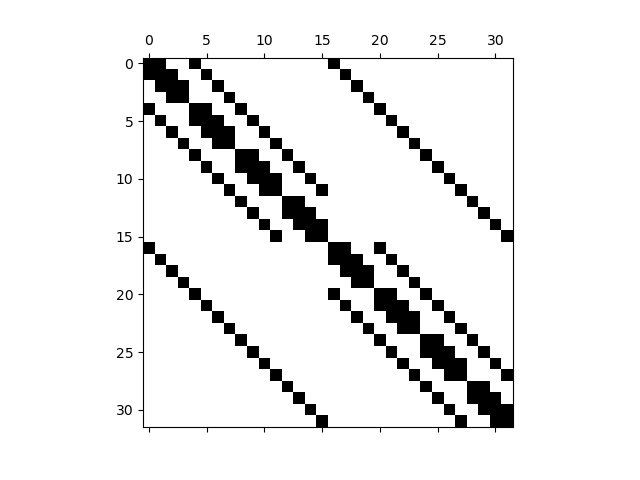
\includegraphics[scale=1.0]{img/spy4.png}
\end{figure}

The size of the resulting matrix scales very rapidly with the domain discretization. A \(100 \times 100\) domain discretization results in a \(20000 \times 20000\) sparse mass matrix to be solved with a direct solution method. For reference, the data visualization of such a matrix looks as seen in the image below, representing an incredibly sparse numerical pattern:

\begin{figure}[H]
    \centering
    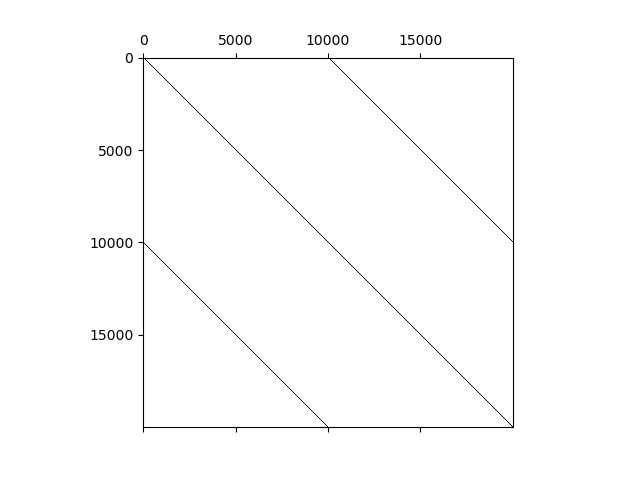
\includegraphics[scale=1.0]{img/spy100.png}
\end{figure}

An iterative solution method may be possible, but typically requires a preconditioned problem and such numerical studies are likely to be outside the scope of the current research domain.

\newpage
\section*{Galerkin Finite Element}
To facilitate the Galerkin finite element solution, we can rewrite the original equations by replacing the terms \(f_i P_i\) and \(g_i P_i\) with \(F_i\) and \(G_i\), respectively. Leaving off the dependence on \(\phi\), \(\theta\), and \(t\) for brevity:

\begin{equation*}
    \frac{\partial P_1}{\partial t} + \frac{\partial F_1}{\partial \phi} + \frac{\partial G_1}{\partial \theta} + \frac{1}{\tau_1} P_1 = \frac{1}{\tau_2} P_2
\end{equation*}

\begin{equation*}
    \frac{\partial P_2}{\partial t} + \frac{\partial F_2}{\partial \phi} + \frac{\partial G_2}{\partial \theta} + \frac{1}{\tau_2} P_2 = \frac{1}{\tau_1} P_1
\end{equation*}

We begin by establishing the equations including basis functions \(v\) and \(w\):

\begin{equation*}
    \int \int v\left(\phi\right) w\left(\theta\right) P_1 \left(\phi, \theta\right) d\phi d\theta
\end{equation*}

\begin{equation*}
    \int \int v\left(\phi\right) w\left(\theta\right) P_2 \left(\phi, \theta\right) d\phi d\theta
\end{equation*}

As well as for the multiphysics terms in \(\phi\) discretization:

\begin{equation*}
    \int \int v\left(\phi\right) \frac{\partial F_1}{\partial \phi} d\phi d\theta
\end{equation*}

\begin{equation*}
    \int \int v\left(\phi\right) \frac{\partial F_2}{\partial \phi} d\phi d\theta
\end{equation*}

And the multiphysics terms in \(\theta\) discretization:

\begin{equation*}
    \int \int w\left(\theta\right) \frac{\partial G_1}{\partial \theta} d\phi d\theta
\end{equation*}

\begin{equation*}
    \int \int w\left(\theta\right) \frac{\partial G_2}{\partial \theta} d\phi d\theta
\end{equation*}

This simplifies to an equation consisting of a constant mass-matrix term, subscripted by the section of domain it appears in. For the \(F_i\) terms:

\begin{equation*}
    M_\theta \int_{\phi_L}^{\phi_R} v\left(\phi\right) \frac{\partial F_1}{\partial \phi} d\phi
\end{equation*}

\begin{equation*}
    M_\theta \int_{\phi_L}^{\phi_R} v\left(\phi\right) \frac{\partial F_2}{\partial \phi} d\phi
\end{equation*}

And for the \(G_i\) terms:

\begin{equation*}
    M_\phi \int_{\theta_B}^{\theta_T} w\left(\theta\right) \frac{\partial G_1}{\partial \theta} d\theta
\end{equation*}

\begin{equation*}
    M_\phi \int_{\theta_B}^{\theta_T} w\left(\theta\right) \frac{\partial G_2}{\partial \theta} d\theta
\end{equation*}

Integrating by parts results in the following terms:

\begin{equation*}
    M_\theta \left(v\left(\phi\right)F_1\left(\phi\right)\rvert_{\phi_L}^{\phi_R} - \int v^\prime\left(\phi\right) F_1\left(\phi\right) d\phi\right)
\end{equation*}

\begin{equation*}
    M_\theta \left(v\left(\phi\right)F_2\left(\phi\right)\rvert_{\phi_L}^{\phi_R} - \int v^\prime\left(\phi\right) F_2\left(\phi\right) d\phi\right)
\end{equation*}

\begin{equation*}
    M_\phi \left(w\left(\theta\right)G_1\left(\theta\right)\rvert_{\theta_B}^{\theta_T} - \int w^\prime\left(\phi\right) G_1\left(\theta\right) d\theta\right)
\end{equation*}

\begin{equation*}
    M_\phi \left(w\left(\theta\right)G_2\left(\theta\right)\rvert_{\theta_B}^{\theta_T} - \int w^\prime\left(\theta\right) G_2\left(\theta\right) d\theta\right)
\end{equation*}

In these equations, we can identify individual components for computation. For example, taking the first equation, it can be rewritten according to:

\begin{equation*}
    v\left(\phi_R\right)F_1\left(\phi_R\right) = L
\end{equation*}

\begin{equation*}
    v\left(\phi_L\right)F_1\left(\phi_L\right) = V
\end{equation*}

Taking note that in the upwinding sense of defining \(V\), \(\phi_L\) is equivalent to \(\phi_R\) from the previous cell.

\begin{equation*}
    \int_{\phi_L}^{\phi_R} v^\prime\left(\phi\right) F_1\left(\phi\right) d\phi = C
\end{equation*}

Resulting in, with cellular indices as subscripts:

\begin{equation*}
    M_\theta \left(L - C\right)_{i,j} - M_\theta V_{i-1,j}
\end{equation*}

Now take note that the general form of \(\mathbf{M}\) is as follows:

\begin{equation*}
    \mathbf{M} = M_\phi \otimes M_\theta
\end{equation*}

A two-by-two discretization domain would result in the following matrix form:

\begin{equation*}
    \mathbf{M} =
    \begin{bmatrix}
        M_{0,0} & 0 & 0 & 0 \\
        0 & M_{1,0} & 0 & 0 \\
        0 & 0 & M_{0,1} & 0 \\
        0 & 0 & 0 & M_{1,1}
    \end{bmatrix}
\end{equation*}

We can use this substitution into the full equation, with similar steps for the \(G_1\) terms:

\begin{equation*}
    \left(M + \left(L - C\right)_\phi + \left(L - C\right)_\theta + \frac{1}{\tau_1}M\right) \vec{P}_1 - \frac{1}{\tau_2}M \vec{P}_2 = V_\phi \vec{P}_1 + V_\theta \vec{P_1}
\end{equation*}

Incorporating a backward Euler substitution with superscripted index \(n\):

\begin{multline*}
    \left(\frac{1}{\Delta t} M + \left(L - C\right)_\phi + \left(L - C\right)_\theta + \frac{1}{\tau_1} M\right) \vec{P}_1^{n+1} - \frac{1}{\tau_2}M \vec{P}_2^{n+1} \\= V_\phi \vec{P}_1^{n+1} + V_\theta \vec{P_1}^{n+1} + \frac{1}{\Delta t} M \vec{P}_1^{n}
\end{multline*}

\begin{multline*}
    \left(\frac{1}{\Delta t} M + \left(L - C\right)_\phi + \left(L - C\right)_\theta + \frac{1}{\tau_2} M\right) \vec{P}_2^{n+1} - \frac{1}{\tau_1}M \vec{P}_1^{n+1} \\= V_\phi \vec{P}_2^{n+1} + V_\theta \vec{P_2}^{n+1} + \frac{1}{\Delta t} M \vec{P}_2^{n}
\end{multline*}

We can again simplify terms:

\begin{equation*}
    \left(L - C\right)_\phi + \left(L - C\right)_\theta - V_\phi - V_\theta = Q
\end{equation*}

Resulting in:

\begin{equation*}
    \begin{bmatrix}
        \left(\frac{1}{\Delta t} - \frac{1}{\tau_1}\right) M + Q_1 & -\frac{1}{\tau_2} M \\
        -\frac{1}{\tau_1}M & \left(\frac{1}{\Delta t} - \frac{1}{\tau_2}\right)M + Q_2
    \end{bmatrix}
    \begin{bmatrix}
        P_1 \\
        P_2
    \end{bmatrix}^{n+1}
    =
    \begin{bmatrix}
        \frac{1}{\Delta t} M & 0 \\
        0 & \frac{1}{\Delta t}
    \end{bmatrix}
    \begin{bmatrix}
        P_1 \\
        P_2
    \end{bmatrix}^n
\end{equation*}

This is approachable by multiplying through from the left by:

\begin{equation*}
    \begin{bmatrix}
        \frac{1}{\Delta t}M & 0 \\
        0 & \frac{1}{\Delta t} M
    \end{bmatrix}^{-1}
\end{equation*}

The main bulk of this construction consists of using appropriate basis functions to form \(C\), \(L\), and \(V\), which collectively form the terms \(Q_i\).

\end{document}
